\documentclass[11pt,letterpaper]{exam}
\usepackage{../study_session}
\usepackage{tikz}
\usetikzlibrary{positioning}

\pagestyle{headandfoot}
\runningheadrule
\firstpageheadrule

\firstpageheader{COMP 2402}{Study Session Practice Questions}{\today}
\runningheader{COMP 2402}{Study Session Practice Questions}{Page \thepage\ of \numpages}
\runningfooter{}{}{}

\title{COMP 2402 Abstract Data Types and Algorithms}
\author{Study Session Questions}

\begin{document}
\maketitle
\vspace{1em}

\section*{Learning Objectives}

\begin{itemize}
\item You should be confident analyzing array-based structures, including
\texttt{ArrayList}, \texttt{Queue}/\texttt{Deque}, \texttt{DualArrayDeque}, and \texttt{RootishArrayStack}.

\item You should be confident analyzing linked list structures, including
\texttt{SLL}/\texttt{DLL}, \texttt{SEList}, and \texttt{SkipList}.

\item You should be confident analyzing tree-based structures, including
\texttt{RandomBSTs}, \texttt{Scapegoat Trees}, \texttt{2-4}/\texttt{Red-Black Trees}, and \texttt{Treaps}.

\item You should be confident analyzing other core structures, including
\texttt{Heaps}, \texttt{Graphs}, \texttt{PriorityQueues}, \texttt{Tries}, and \texttt{HashTables}.

\item You should be comfortable with runtime and amortized analysis for these data structures and sorting algorithms.
\end{itemize}

\section*{I. Array-Based Lists}

\begin{itemize}
\item Contiguous blocks of memory - easy O(1) access to values
\item Adding or removing in the middle of a list requires shifting elements - variable runtimes
\item Cannot expand or shrink without allocating a new array and copying values to new array - expensive!
\end{itemize}

\begin{questions}

\mcquestion{If we resize a backing array in an \texttt{ArrayStack} via \texttt{grow()}, what conclusion can be drawn?}{
\choice At least $\frac{n}{2}$ \texttt{add()} operations have occured since then
\choice At least $\frac{2n}{3}$ \texttt{remove()} operations have occured since then
\choice At least $\frac{2n}{3}$ \texttt{add()} operations have occured since then
\choice At least $\frac{n}{2}$ \texttt{remove()} operations have occured since then
\choice We cannot bound the number of \texttt{add()} nor \texttt{remove()} operations
}

\mcquestion{Recall that we shrink the backing array $a$ when $3n < a.\texttt{length}$. If we are currently about to shrink the array...}{
\choice At least $\frac{n}{2}$ \texttt{add()} operations have occured since then
\choice At least $\frac{2n}{3}$ \texttt{remove()} operations have occured since then
\choice At least $\frac{2n}{3}$ \texttt{add()} operations have occured since then
\choice At least $\frac{n}{2}$ \texttt{remove()} operations have occured since then
\choice We cannot bound the number of \texttt{add()} nor \texttt{remove()} operations
}

\mcquestion{What is the minimum number of elements a \texttt{RootishArrayStack} of block size 9 can hold without needing to shrink?}{
\choice 28
\choice 29
\choice 36
\choice 37
\choice 45
\choice 46
}

\mcquestion{In a \texttt{RootishArrayStack}, what will a call to \texttt{get(10)} (get the element with index 10) return?}{
\choice \texttt{blocks.get(0)[10]}
\choice \texttt{blocks.get(5)[1]}
\choice \texttt{blocks.get(3)[4]}
\choice \texttt{blocks.get(4)[0]}
\choice \texttt{blocks.get(4)[1]}
\choice \texttt{blocks.get(4)[4]}
}

\mcquestion{A \texttt{DualArrayDeque} uses two \texttt{ArrayStacks}, \texttt{front} and \texttt{back}. What's the implementation for \texttt{get(i)} ?}{
\choice A: \texttt{front.get(i)}
\choice Either A or B depending on the value of $i$ and \texttt{front.size()}
\choice B: \texttt{front.get(front.size() - i - 1)}
\choice Either A or C depending on the value of $i$ and \texttt{front.size()}
\choice C: \texttt{back.get(i - front.size())}
\choice Either B or C depending on the value of $i$ and \texttt{front.size()}
}

\shortanswer[1.25in]{Explain amortization in your own words.}

\section*{II. LinkedList Structures}

\begin{itemize}
\item Rather than O(1) access we must walk through the list, one at a time, until the ith element is reached
\item Easier insertion and deletion
\end{itemize}

\question Which of the following methods are usually \textbf{much faster} on a LinkedList versus an ArrayList? Select all that apply.
\begin{checkboxes}
\choice read the first element of a list $n$ times
\choice read a newly-randomly-indexed element of the list $n$ times
\choice insert $n$ elements at the end of a list
\choice insert $n$ elements at the beginning of a list
\choice insert $n$ elements at index $\frac{size}{2}$ (which doesn't change)
\choice none of these
\end{checkboxes}

\mcquestion{Consider a SEList with $b = 5$. The last element of the last block has index 14. How many blocks \textit{could} the list have?}{
\choice two
\choice three
\choice four
\choice five
\choice six
\choice seven
}

\mcquestion{In a Doubly-Linked List, how is traversal direction optimized in \texttt{getNode(i)} ?}{
\choice The list will randomly traverse from the head or tail to amortize speed
\choice The list always traverses from head to save space
\choice The list always traverses from tail to save space
\choice A recursive traversal is implemented
\choice The direction (head or tail) depends on the value of $i$
}

\question Which of the following statements are true with regards to SkipLists? Select all that apply.
\begin{checkboxes}
\choice The expected time complexity of \texttt{get(i)} is $O(\log n)$.
\choice The worst-case time complexity of a find operation is $O(n^2)$.
\choice The level/height of a node in a SkipList is determined by random chance.
\choice The "sentinel" node in a SkipList always holds the largest element.
\choice The maximum level of any node grows as $O(\log n)$.
\choice The expected time complexity of finding the last element is $O(1)$.
\end{checkboxes}

\shortanswer[1.25in]{Explain the role of the dummy node. In particular, what are dummy.next and dummy.prev?}

\section*{Part III - Trees -}

\begin{quote}
"If you want to know why the tree grows upside down, ask the computer scientists who introduced this convention. (The conventional wisdom is that they never went out of the room and so they never saw a real tree.)"
\end{quote}

\question Match each type of tree with its corresponding description.
\begin{matching}
\mitem{A}{Treap}{1}{randomized balancing with expected $O(\log n)$ performance using priorities}
\mitem{B}{Scapegoat Tree}{2}{maintains balance by rebuilding entire subtrees when imbalance is detected}
\mitem{C}{Red-Black Tree}{3}{binary implementation of a 2-4 tree, guaranteed $O(\log n)$ height}
\mitem{D}{2-4 Tree}{4}{fewest tree levels by allowing multi-key nodes, multiple splits per step}
\end{matching}

\newpage

\question If we \texttt{add(19)}, then \texttt{removeMin()} to the heap below, what will the heap look like afterwards as an array?

\begin{center}
\texttt{15, 23, 18, 45, 49, 33, 25, 56, 62, 50}

\vspace{0.75em}

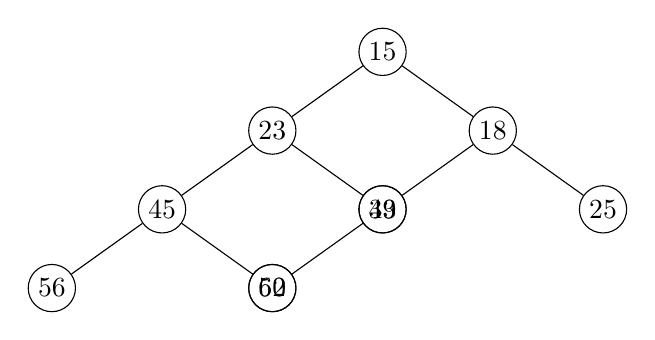
\begin{tikzpicture}[
  level distance=10mm,
  sibling distance=28mm,
  every node/.style={circle,draw,minimum size=6mm,inner sep=0pt},
  edge from parent/.style={draw}
]
\node{15}
child{
  node{23}
  child{
    node{45}
    child{node{56}}
    child{node{62}}
  }
  child{
    node{49}
    child{node{50}}
    child[missing]
  }
}
child{
  node{18}
  child{node{33}}
  child{node{25}}
};
\end{tikzpicture}
\end{center}

\begin{choices}
\choice \texttt{[19, 18, 25, 45, 50, 33, 49, 56, 62, 23]}
\choice \texttt{[23, 18, 45, 49, 33, 25, 56, 62, 50, 19]}
\choice \texttt{[18, 19, 25, 45, 23, 33, 49, 56, 62, 50]}
\choice \texttt{[18, 23, 19, 25, 33, 45, 49, 50, 56, 62]}
\choice \texttt{[18, 19, 45, 23, 33, 25, 56, 62, 50, 49]}
\choice none of these
\end{choices}

\question Match each type of tree traversal with its implementation.
\begin{matching}
\mitem{A}{preorder}{1}{Visit root, then left subtree always, then right subtree.}
\mitem{B}{inorder}{2}{Visit left subtree, root, then right subtree.}
\mitem{C}{postorder}{3}{Visit from the leaves to the root, prioritizing left subtrees first}
\mitem{D}{breadth-first}{4}{Visit level by level, from root to leaves, prioritizing left subtrees}
\end{matching}

\mcquestion{What is the time complexity to rebuild a subtree of size $s$ in a scapegoat tree?}{
\choice $O(1)$
\choice $O(\log s)$
\choice $O(s \log s)$
\choice $O(s)$
\choice $O(s^2)$
\choice $O(2^s)$
}

\mcquestion{In a 2-4 tree, what happens when inserting a key causes a node to exceed its maximum of 3 keys (i.e., 4 children)?}{
\choice The tree is restructured from the root down to evenly redistribute all keys
\choice The node's subtree is rebalanced by rotating keys with siblings
\choice The node is split into two nodes, and the middle key is promoted to parent
\choice The insertion is deferred until the next rebalancing phase
}

\section*{IV. Everything Else}

\begin{itemize}
\item Graphs: Nodes with edge links
\item BinaryTries: prefix tree for binary strings
\item HashTables: Key-value store via hash formula
\item MeldableHeap: heap w/ random merge path
\item PriorityQueues: Remove item with top rank
\end{itemize}

\mcquestion{Recall \[
h(x) = ((z \cdot x) \bmod 2^w)\ \mathrm{div}\ 2^{w-d}
\]
Suppose $w = 5, d = 3, z = 9$. What is $h(6)$ ?}{
\choice $h(6) = 2$
\choice $h(6) = 3$
\choice $h(6) = 4$
\choice $h(6) = 5$
\choice $h(6) = 6$
\choice $h(6) = 7$
}

\question Put the following steps in correct order for melding two heaps $h1$ and $h2$.
\begin{enumerate}
\item If one heap is empty, return the other
\item Compare root values of $h1$ and $h2$
\item Swap $h1$ and $h2$ if $h2$ has a smaller root
\item Recursively meld $h1$'s right child with $h2$
\end{enumerate}
\vspace{0.5em}
\fillwithlines{1.0in}

\question Perform a BFS on this graph, starting from 0. Indicate the order of vertices traversed (i.e. 0 1 2 3 4 5)

\begin{center}
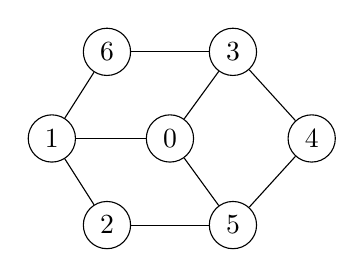
\begin{tikzpicture}[
  every node/.style={circle,draw,minimum size=6mm,inner sep=0pt},
  node distance=20mm
]
\node (n6) at (0,1.5) {6};
\node (n3) at (1.6,1.5) {3};
\node (n1) at (-0.7,0.4) {1};
\node (n0) at (0.8,0.4) {0};
\node (n4) at (2.6,0.4) {4};
\node (n2) at (0.0,-0.7) {2};
\node (n5) at (1.6,-0.7) {5};

\draw (n6) -- (n1);
\draw (n6) -- (n3);
\draw (n1) -- (n0);
\draw (n1) -- (n2);
\draw (n0) -- (n3);
\draw (n0) -- (n5);
\draw (n2) -- (n5);
\draw (n3) -- (n4);
\draw (n5) -- (n4);
\end{tikzpicture}
\end{center}

\fillwithlines{0.75in}

\mcquestion{If $x$ is not in a \texttt{BinaryTrie}, what does \texttt{find(x)} do?}{
\choice Returns null
\choice Returns a random key
\choice Finds the smallest key greater than $x$
\choice Finds the root value
}

\mcquestion{In a chained hash table, what happens when two keys hash to the same index?}{
\choice One key is discarded
\choice A binary search tree is created
\choice Both are stored in a linked list at that slot
\choice A hash collision error is thrown
}

\section*{V. Sorting Algorithms and Runtime Efficiency}

No description

\question Place the following runtime complexities in order of relative growth, starting with the slowest.
\begin{itemize}
\item $O(\log n)$
\item $O(n)$
\item $O(n \log n)$
\item $O(n^2)$
\end{itemize}
\vspace{0.5em}
\fillwithlines{1.0in}

\mcquestion{How does QuickSort work?}{
\choice Splits array in half and merges sorted parts
\choice Repeatedly selects minimum and moves it to front
\choice Picks a pivot, partitions array, recursively sorts parts
\choice Builds a heap and extracts elements one by one
}

\mcquestion{What is the space complexity of MergeSort (recall that it is not in-place)?}{
\choice $O(1)$
\choice $O(\log n)$
\choice $O(n)$
\choice $O(n \log n)$
}

\mcquestion{What is the time complexity of HeapSort in the worst case?}{
\choice $O(\log n)$
\choice $O(n)$
\choice $O(n \log n)$
\choice $O(n^2)$
}

\question How much more review do you think you'll have to do for the exam?

none at all / a lot more

\end{questions}

\end{document}
